\documentclass{article}
\usepackage{graphicx}
\usepackage{amsthm}
\usepackage{amsfonts}
\usepackage{amsmath}
\usepackage{amssymb}
\usepackage{fullpage}
\usepackage[usenames]{color}
\usepackage{hyperref}
  \hypersetup{
    colorlinks = true,
    urlcolor = blue,       % color of external links using \href
    linkcolor= blue,       % color of internal links 
    citecolor= blue,       % color of links to bibliography
    filecolor= blue,        % color of file links
    }
    
\usepackage{listings}

\definecolor{dkgreen}{rgb}{0,0.6,0}
\definecolor{gray}{rgb}{0.5,0.5,0.5}
\definecolor{mauve}{rgb}{0.58,0,0.82}

\lstset{frame=tb,
  language=haskell,
  aboveskip=3mm,
  belowskip=3mm,
  showstringspaces=false,
  columns=flexible,
  basicstyle={\small\ttfamily},
  numbers=none,
  numberstyle=\tiny\color{gray},
  keywordstyle=\color{blue},
  commentstyle=\color{dkgreen},
  stringstyle=\color{mauve},
  breaklines=true,
  breakatwhitespace=true,
  tabsize=3
}

\theoremstyle{theorem} 
   \newtheorem{theorem}{Theorem}[section]
   \newtheorem{corollary}[theorem]{Corollary}
   \newtheorem{lemma}[theorem]{Lemma}
   \newtheorem{proposition}[theorem]{Proposition}
\theoremstyle{definition}
   \newtheorem{definition}[theorem]{Definition}
   \newtheorem{example}[theorem]{Example}
\theoremstyle{remark}    
  \newtheorem{remark}[theorem]{Remark}


\title{CPSC-406 Report}
\author{Everett Prussak  \\ Chapman University}

\date{\today}

\begin{document}

\maketitle

\begin{abstract}
Consisting of CPSC 406 Material at Chapman University with Professor Alexander Kurz. This report will include an Introduction, Weekly Homework, and a Paper on the group project, which is done throughout the semester. 
\end{abstract}

\tableofcontents

\section{Introduction}\label{intro}
This report...

\section{Homework}\label{homework}

This section contains solutions to homework. 

\subsection{Week 2 (Homework 1)}
This week's homework was to solve the following NFA:\noindent\newline
\includegraphics[scale=0.8]{a}\noindent\newline
\noindent\newline This is the following NFA but drawn out:

\includegraphics[scale=0.2]{nfa}\noindent\newline

From this NFA, the following DFA table can be made:\noindent\newline
\includegraphics[scale=0.8]{b}\noindent\newline

\includegraphics[scale=0.2]{dfa}\noindent\newline

\noindent\newline\newline This DFA diagram will allow for the correct initial state, final states, and correct path for each input.


\subsection{Week 3 (Homework 2)}
\noindent Week 3 consisted of 2 Questions. They are in their respective sections.\newline

\subsubsection{Question 1}
For Week 3 Question the object was to write the steps of the unification algorithm for each pair. \newline

\includegraphics[scale=0.75]{c}\noindent\newline

\noindent\newline For number 1 of question 1 I got the following answer:

\begin{verbatim}
1. f(X,f(X,Y)) = f(f(Y,a),f(U,b))

  1. X = f(Y,a)
      o1 = [f(Y,a)/X]

  2. f(X,Y) = f(U,b)
      3. X = U
          o3 = [U/X]
      4. Y = b
          o4 = [b/Y]

  5. X(o3 * o4) = U, f(o3 * o4)(Y,a) = f(b,a)
      U = f(b, a)
      o5 = [f(b,a)/U]


o = o3 * o4 * o5 = [U/X, b/Y, f(b,a)/U]
X = U, Y = b, U = f(b,a)
\end{verbatim}

\noindent\textbf{Note: Sigma Symbol was not working in Verbatim, thus a simple lowercase o was subsitituted.}

\noindent\newline\newline For number 2 of question 1 I got the following answer:

\begin{verbatim}
2. f(g(U),f(X,Y)) = f(X,f(Y,U))

  1. g(U) = X
       o1 = [g(U)/X]

  2. f(X,Y) = f(Y,U)
       3. X = Y
          o3 = [Y/X]
       4. Y = U
          o4 = [U/Y]

o = o1 * o2 * o3 = [X/U, Y/X, g(Y)/Y]
\end{verbatim}

\noindent\newline\newline For number 3 of question 1 I got the following answer:
\begin{verbatim}
3. h(U,f(g(V),W),g(W)) = h(f(X,b),U,Z)

  1. U = f(X,b)
     o1 = [f(X,b)/U]

  2. f(g(V),W) = U
     o2 = [f(g(V),W)/U]

  3. g(W) = Z
     o3 = [g(W)/Z]

  4. U(o1 * o2) --> f(X,b) = f(g(V),W)

     5. X = g(V)
        o5 = [g(V)/X]

     6. b = W
        o6 = [b/W]

  7. Z(o3 * o6) = g(W), W = b
     o7 = [g(b)/Z]

  8. U(o1 * o2 * o6) --> f(X,b) = f(g(V), b)
     o8 [f(g(V),b)/U]


  o = o5 * o6 * o7 * o8 = [f(g(V),b)/U, g(V)/X, b/W, g(b)/Z]


  U = f(g(V),b), W = b, X = g(V), Z = g(b)
\end{verbatim}

\subsubsection{Question 2}
For question 2, the task was to draw a SLD Recursion Tree for the following:\newline
\includegraphics[scale=0.65]{f}\newline\newline\newline

\noindent I got the following SLD Tree:
\begin{verbatim}



                   twoway(W,a)
                  /           \
                 /             \
              conn(W,a)        conn(a,W)
              /        \        /       \
            W=b        W=d   W=c       no
                        |            /  |  \
                        no          b   d   c
\end{verbatim}

\noindent\newline twoway(W,a) becomes conn(W,a) and conn(a,W) because of the rule twoway(X,Y):- conn(X,Y), conn(Y,X). This becomes the first part of the tree. Then for the conn(X,Y), it becomes conn(W,a). This side of the tree will split into W=b and W=d. W=d eventually fails because there is no serv(d). However, W=b is successful because we have addr(a,b) and a a serv(b), which allows for the conn(b,a) to be true. On the right side of the tree, we have conn(a,W). This will split into w=c and no. Since c holds the address of a, and b holds the address of c, and serv(b) exists, we can create a conn(a,c) because of these factors. We see in the equation addr(X,Z), serv(Z), addr(Z,Y) can be applied here. In our case it would look similar to addr(a,b) serv(b) addr(b,c), which allows conn(b,c) to be true.


\subsection{Week 6 (Homework 3)}
\noindent\newline The goal this week was to solve the following:

\includegraphics[scale=0.64]{abcd}\noindent\newline

\noindent\newline I split this into to two parts (Top and Bottom Questions).

\subsubsection{Part 1 (Top)}
\noindent\newline Here is my answer for number 1:

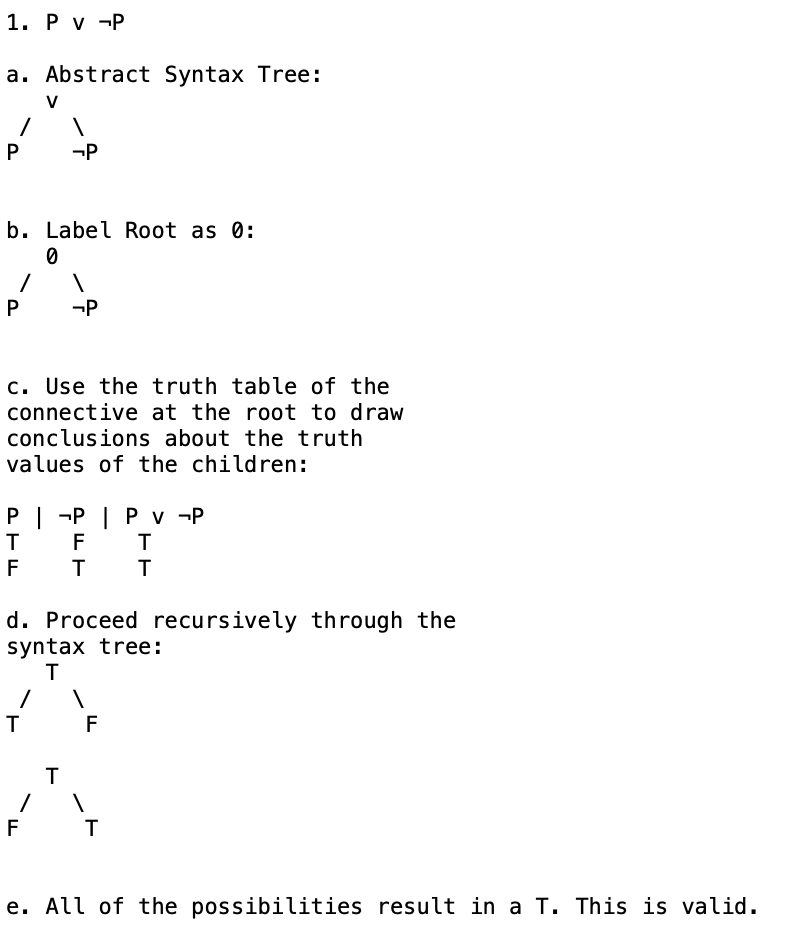
\includegraphics[scale=0.64]{hw6_1}\noindent\newline

\noindent\newline Here is my answer for number 2:

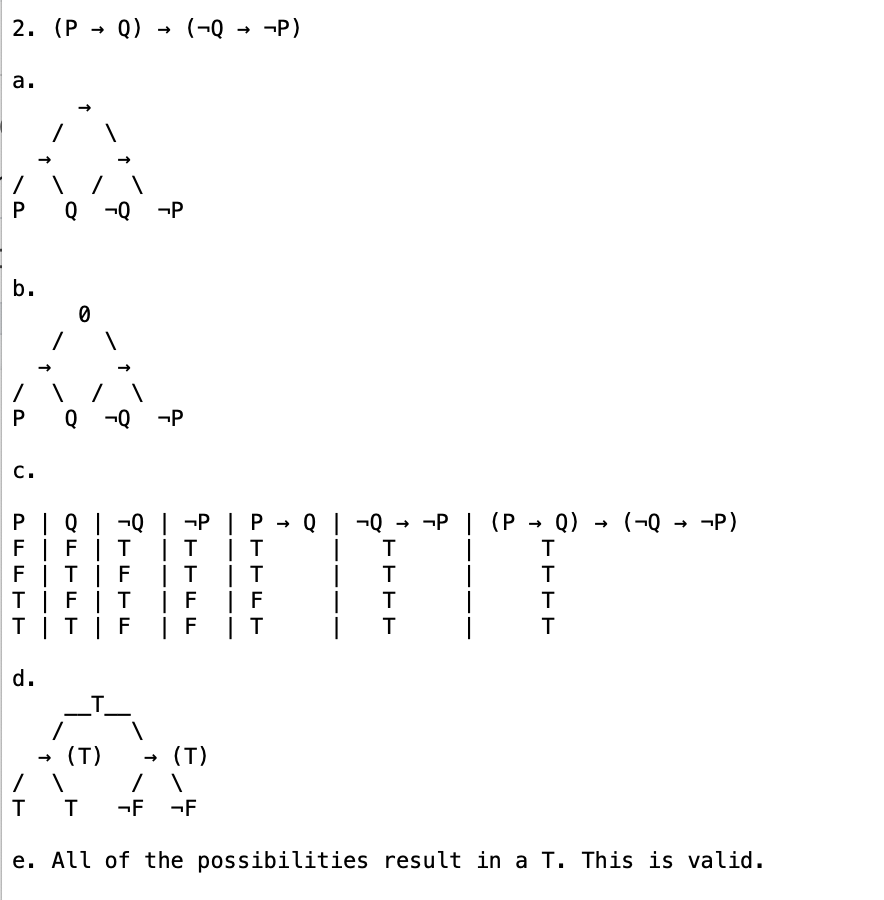
\includegraphics[scale=0.64]{hw6_2}\noindent\newline

\noindent\newline Here is my answer for number 3:

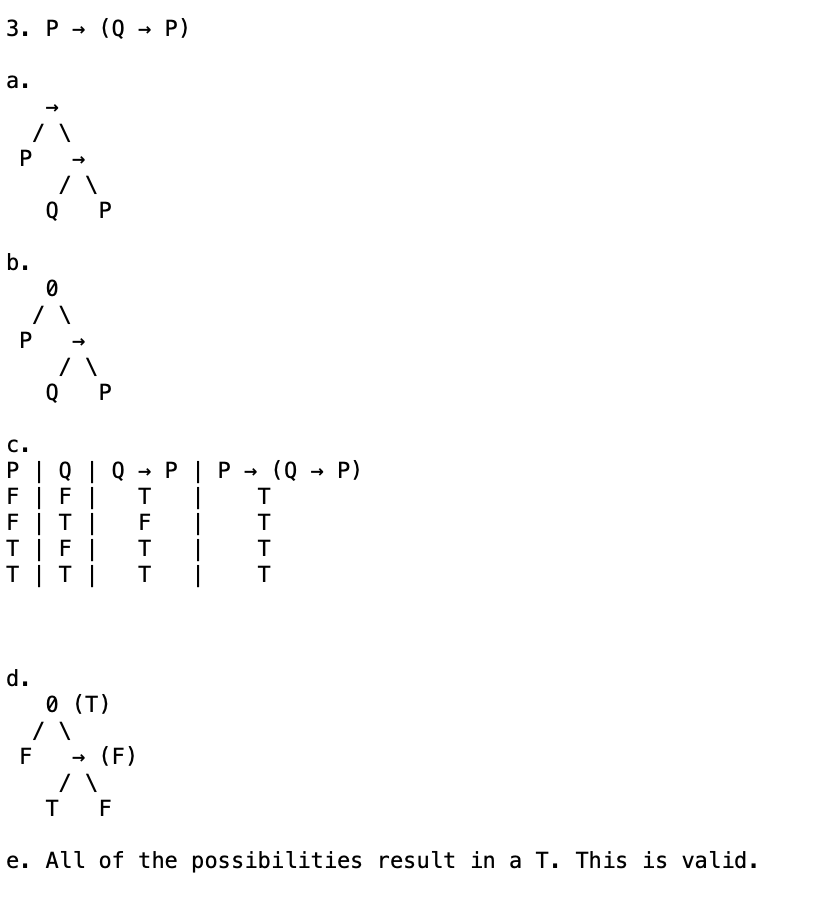
\includegraphics[scale=0.64]{hw6_3}\noindent\newline

\noindent\newline Here is my answer for number 4:

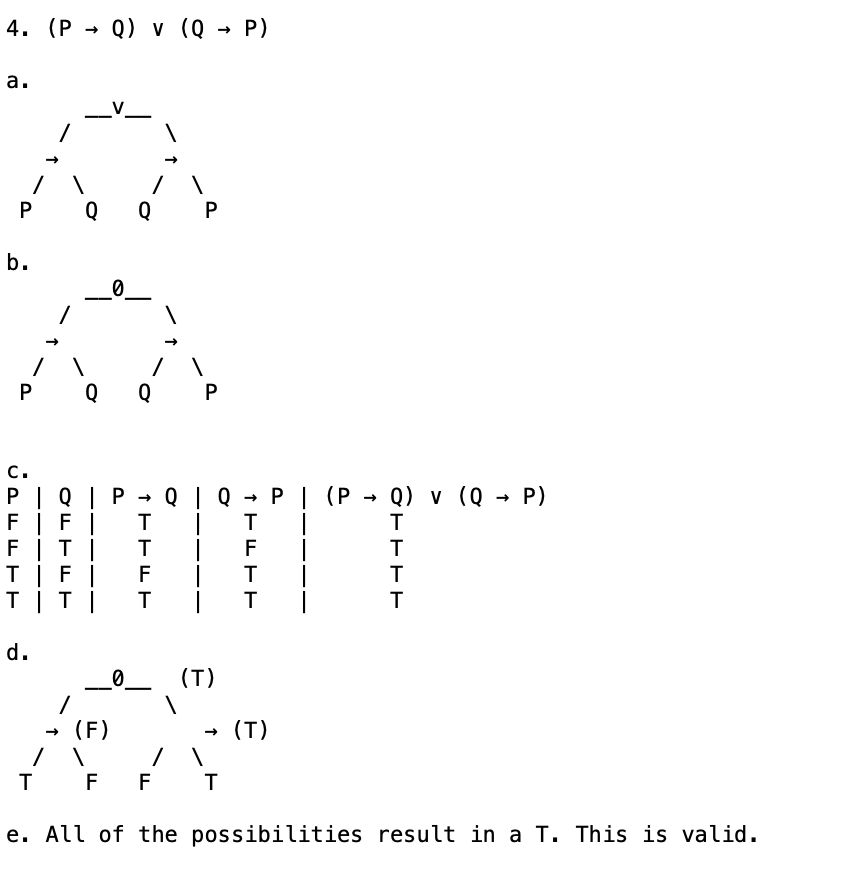
\includegraphics[scale=0.64]{hw6_4}\noindent\newline

\noindent\newline Here is my answer for number 5:

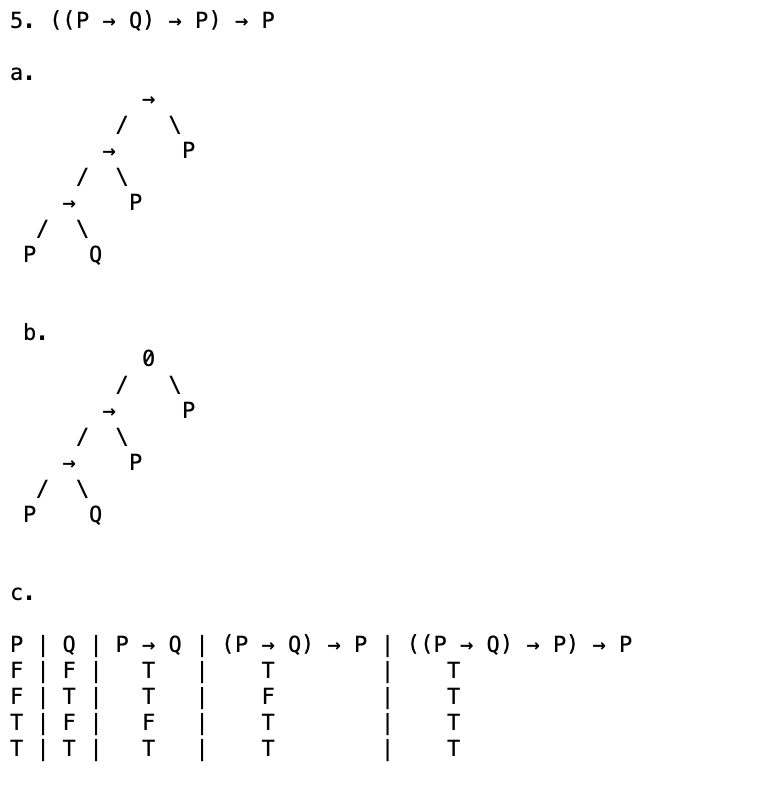
\includegraphics[scale=0.64]{hw6_5_1}\noindent\newline
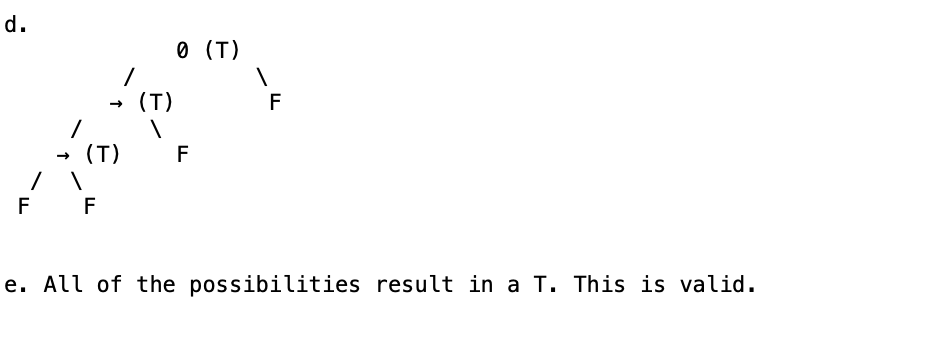
\includegraphics[scale=0.64]{hw6_5_2}\noindent\newline

\noindent\newline Here is my answer for number 6:

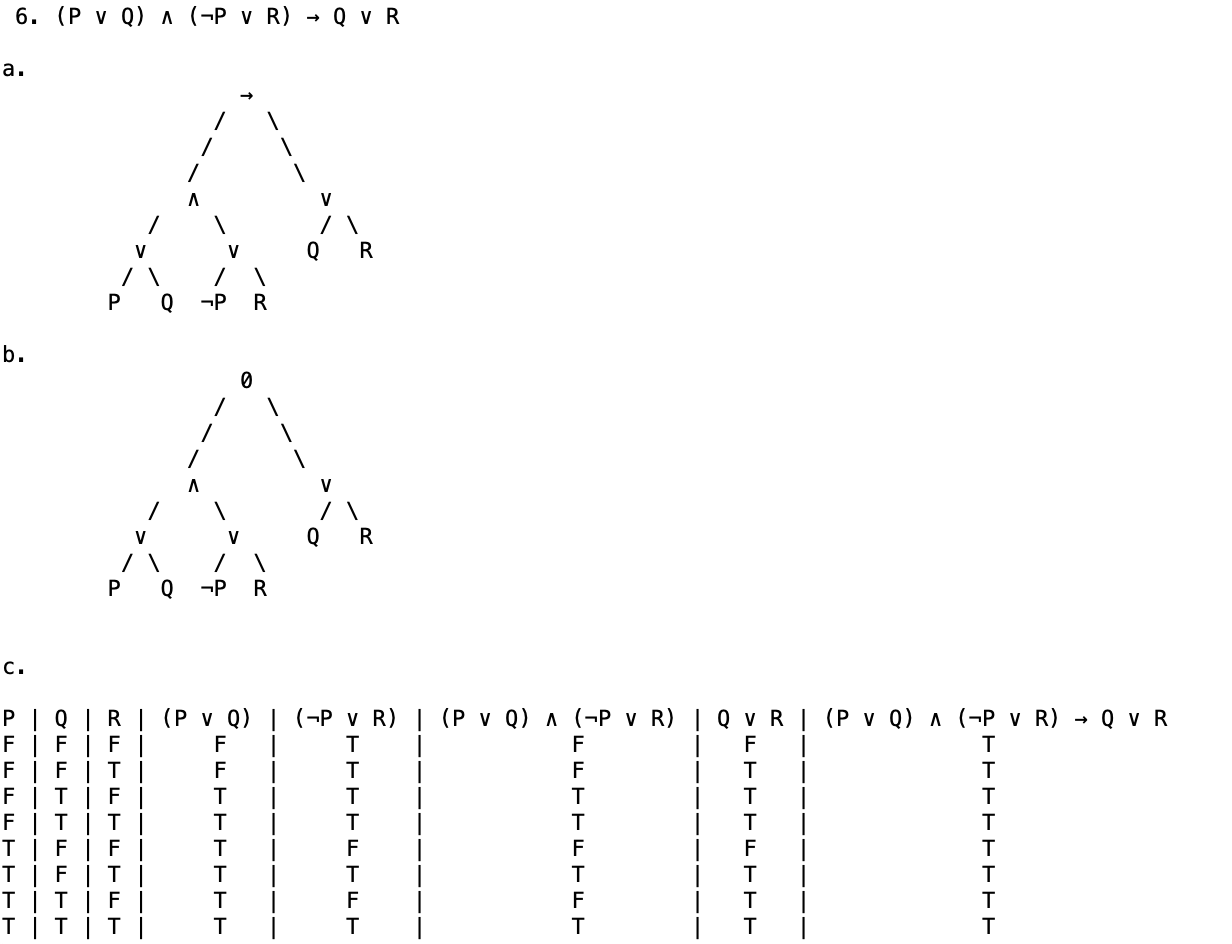
\includegraphics[scale=0.64]{hw6_6}\noindent\newline
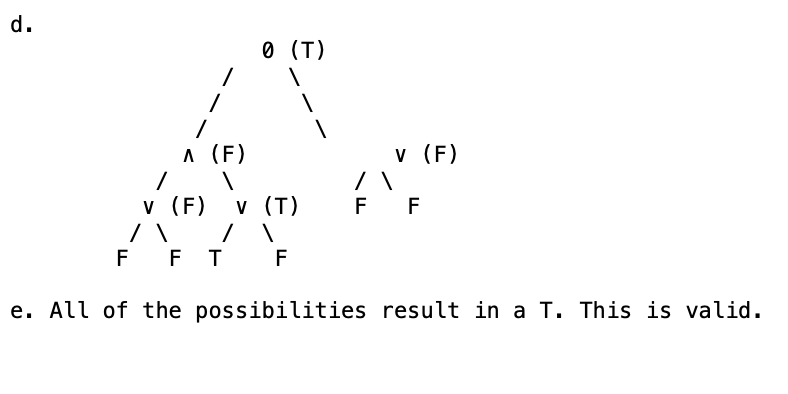
\includegraphics[scale=0.64]{hw6_6_2}\noindent\newline

\subsubsection{Part 1 (Bottom)}
\noindent\newline Here is my answer for number 1:

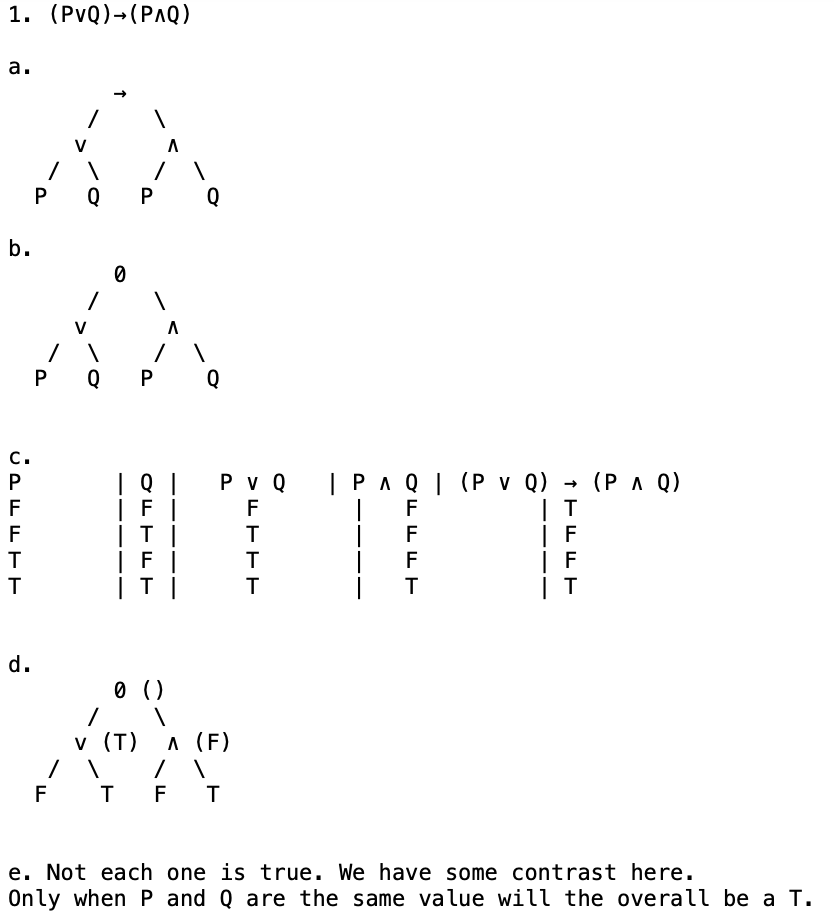
\includegraphics[scale=0.64]{hw6_bottom_1}\noindent\newline

\noindent\newline Here is my answer for number 2:

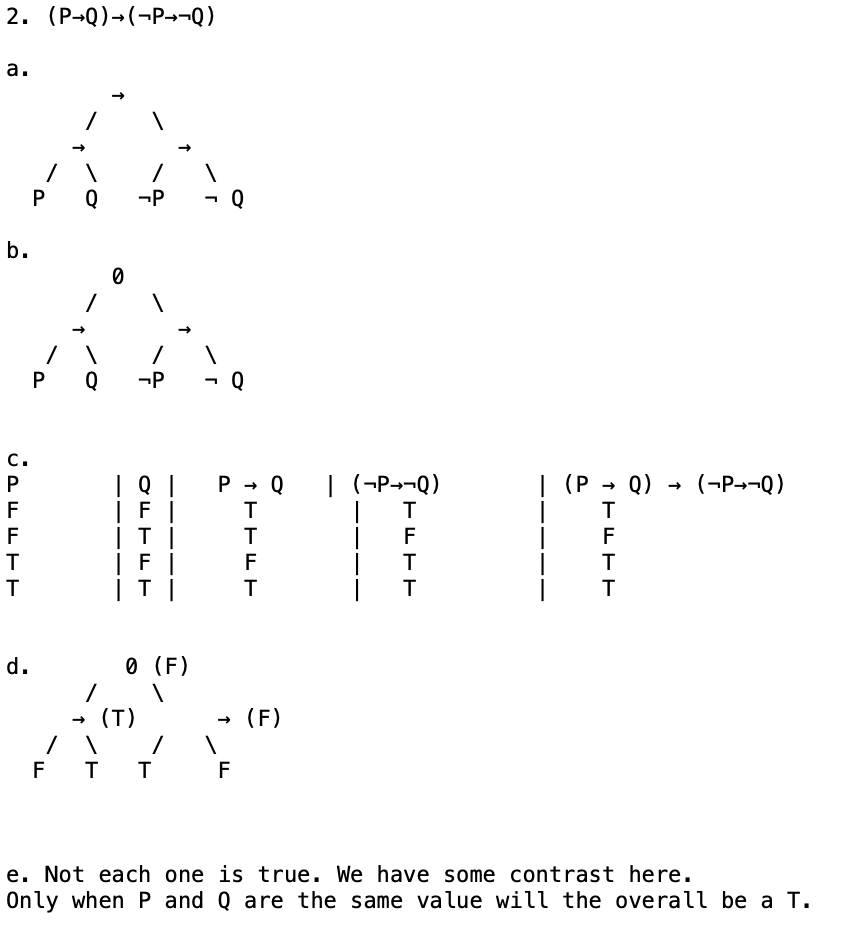
\includegraphics[scale=0.64]{hw6_bottom_2}\noindent\newline


\noindent Note: I had trouble converting some of the symbols I used in my .txt file in my Verbatim. I used many screenshots instead. I will add my .txt and .jpg's in a folder called homeworkMedia on github!


\subsection{Week 9}
This weeks tasks were to experiment with Spin, and solve 4 exercises.

\noindent\newline Formulas:
\begin{verbatim}
[]  (success && bobAlice -> aliceBob)
[]  (success && aliceBob -> bobAlice)
\end{verbatim}


\noindent\newline\textbf{Exercise 1:} 
Go through the program, find these variables, and describe in plain language the meaning of these propositions above.

\noindent\newline The 3 variables that will be discussed are success, bobAlice, and aliceBob. The variable success is a boolean variable. If the protocol runs to completion, then it will be set as 'True'. If it breaks somewhere down the line, then the protocol is not a 'success' and would be set to 'False'. The bobAlice variable is another boolean variable. If Bob receives a message from Alice then it would be set as 'True'. If Bob does not receive a message from Alice then it would be set as 'False'. Lastly, aliceBob is another boolean variable. If Alice receives a message from Bob then it would be set to 'True', if not then it would be 'False'.

\noindent\newline With all of these variables explained, the first formula would read if there is a success in the completion of the protocol and Bob is receives a message from Alice, then Bob is communicating with Alice. The next formula would read if there is a success in the completion of the protocol and Alice is receives a message from Bob, then Alice is communicating with Bob.


\noindent\newline\textbf{Exercise 2:} 
Which of the two formulas (from above) is verified as correct and which one is violated? What do we learn from this about the correctness of the protocol?

The second formula was verified as correct
\begin{verbatim}
[]  (success && aliceBob -> bobAlice)
\end{verbatim}

\noindent\newline While the first formula was violated
\begin{verbatim}
[]  (success && bobAlice -> aliceBob)
\end{verbatim}


\noindent\newline\newline This tells us that the variables \textbf{success} and \textbf{bobAlice} were True boolean variables. The variable \textbf{aliceBob} was False, and this formula would result in violated truth table, with 1 -> 0 being an outcome of 0 as well, meaning violated.

\noindent\newline Relevant Output (Violated Formula):
\begin{verbatim}
spin -a ns.pml; cc -o pan pan.c; ./pan -a

pan:1: assertion violated  
!( !(( !((((statusA==1)&&(statusB==1))&&(partnerB==10)))||(partnerA==9)))) (at depth 83)
pan: wrote ns.pml.trail

\end{verbatim}


\noindent\newline\textbf{Exercise 3:}
The property that is violated produces an execution sequence. How long is that execution sequence?

\noindent\newline The number of execution steps I read from my terminal using this command:
\begin{verbatim}
spin -p -t ns.pml
\end{verbatim}

\noindent was \textbf{84 execution sequences}. 

\noindent\newline Relevant Output:
\begin{verbatim}
vi ns.pml.trail

81:2:41
82:0:116
83:1:20
84:0:113
\end{verbatim}



\noindent\newline\textbf{Exercise 4:}
Use Spin to produce an MSC that represents a successful attack on the protocol. Explain in detail why the MSC constitutes a successful attack.


\noindent\newline These were the new propositional variable I created/used:
\begin{verbatim}
#define success		(statusA == ok && statusB == ok)
#define aliceBob	(partnerA == bob)
#define bobAlice	(partnerB == alice)
#define intruderAlice (partnerB == intruder)
#define intruderBob (partnerA == intruder)
#define bobIntruder (partnerA == bob)
#define aliceIntruder (partnerB== alice)
#define knowNA		(knowNA)
#define knowNB		(knowNB)
#define knownNI   (knowNI)
\end{verbatim}

\noindent\newline These were the formulas/properties I created:
\begin{verbatim}
ltl {[]  (success && aliceIntruder -> intruderAlice)}
ltl {[]  (success && intruderBob -> bobIntruder)}
ltl {[]  (success && bobIntruder -> intruderAlice)}
\end{verbatim}

\noindent\newline This was the output:
\begin{verbatim}
pan: ltl formula ltl_0
\end{verbatim}

\noindent\newline I was slightly confused in how to create a successful attack in Spin, but I believe that this worked and was classified as an \textbf{attack}. First, Alice sends a message to the Intruder. The Intruder then sends a message to Bob, where Bob then sends a message back to the Intruder. This means that the intruder would be able to impersonate both Bob and Alice. In theory, if Alice had access or control of Bob's money, the Intruder could send a message to get Bob's money from Alice by impersonating Bob. This would be a very bad attack on both Alice and Bob.


\noindent\newline To be considered a \textbf{successful attack}, the LTL-correctness properties are to be verified.

\subsection{Week 11}
This week there were two tasks. The first task was to illustrate the following automata:\newline
\includegraphics[scale=0.75]{hw11_a}

\subsubsection{Part 1}
\noindent\newline For this I drew them following automata:\newline
\includegraphics[scale=0.6]{hw11_p1}

\noindent\newline A1 and A2 were the original DFA's. The Top Right (Pink) is the Union, then middle (Purple) is sequential composition, and lastly bottom (Blue) is Kleene Star.

\subsubsection{Part 2}
\noindent\newline The next task were to do the following two exercises. The Regular Expression, DFA, and Epsilon NFA were to be created for each.

\noindent\newline Here are the two exercises:\newline
\includegraphics[scale=0.55]{hw11_b}

\noindent\newline\newline For the first exercise I got the following Regular Expression
\begin{verbatim}
A = {0 + 1+ ... + 9}*

RE: A0A0 + A1A1 + ... + A9A9
\end{verbatim}

\noindent\newline For this regular expression, I created a rule for A. This allowed it to be written easier, and therefore the reader can understand it better.

\noindent\newline\newline For the DFA I created:\newline
\includegraphics[scale=0.75]{hw11_p2dfa}

\noindent\newline\newline For the Epsilon NFA I created:\newline
\includegraphics[scale=1.0]{hw11_p2nfa}

\noindent\newline\newline For the second exercise I got the following Regular Expression
\begin{verbatim}
RE1: a*
RE2: b*
RE3: c*

Final RE: (abc)*
\end{verbatim}

\noindent\newline\newline For the DFA I created:\newline
\includegraphics[scale=0.75]{hw11_p3dfa}

\noindent\newline\newline For the Epsilon NFA I created:\newline
\includegraphics[scale=0.75]{hw11_p3nfa}


\subsection{Week 12}
\noindent\newline This week's homework required an analysis of some Java and Python programs and to dissect them further.

\subsubsection{Number 1}
\noindent\newline Exercise 1: Have a look at peterson.py. What program behavior do you expect? Is your expectation confirmed when you run the program? 

\noindent\newline\newline Before running the program, I would expect for the Counter Value to be 20,000. After running the program my expectation was correct, as the value printed was 20,000.


\subsubsection{Number 2}
\noindent\newline Exercise 2: Analyse the Java program peterson in the same way as you analysed the Python program in the previous exercise. Make sure to run the Java program on your local machine. What observations do you make? 

\noindent\newline\newline Again, I expected the counter value to be 20,000. When running peterson.java inside of the Online Java Website, I received the value of 20,000 each time. However, when I did peterson.java on my local machine I had different results. Interestingly, I would receive numbers close to 20,000 such as 19,912 or 19,930. I never had a counter value of 20,000 when running on my local machine which is very interesting.


\subsubsection{Number 3}
\noindent\newline Exercise 3: Explain why the outcome a = 0, b = 0 is not sequentially consistent, but the other three outcomes are.

\noindent\newline\newline The outcome a = 0 and b = 0 is not sequentially consistent because the program has multiple threads involved, but those threads are not synchronized properly.

\noindent\newline\newline From a more indepth explanation from AI: 
\begin{verbatim}
The threads t1 and t2 can access the shared variables x and y concurrently, and both threads can
update the shared variables a and b. 
The operations of the threads can be interleaved in different ways, leading to different outcomes.

In the case of a = 0, b = 0, the following interleaving of operations is possible:

t1 sets x = 1
t2 sets y = 1 and reads x as 0
t1 reads y as 0 and sets b = y as 0
t2 sets a = x as 0
Therefore, the outcome a = 0, b = 0 violates the sequentially consistent execution of the program.
\end{verbatim}

\subsubsection{Number 4}
\noindent\newline Exercise 4: Report the results you get from running memoryModelWithStats on your local machine. Include the specs of our processor, in particular the number of cores. If you can find out something about the cashes, add this as well. 

\noindent\newline\newline Here are the results from running memoryModelWithStats on my local machine.

\begin{verbatim}
Outcomes after 1000 iterations:
(0, 0): 1
(0, 1): 451
(1, 0): 543
(1, 1): 5
\end{verbatim}

\noindent\newline\newline Here is the information about my Mac's Processor and the number of cores:
\begin{verbatim}
Processor Name:  Dual-Core Intel Core i3
Processor Speed:  1.1 GHz
Number of Processors:  1
otal Number of Cores:  2
\end{verbatim}

\subsubsection{Number 5}
\noindent\newline Exercise 5: You can force sequential consistency of memoryModelWithStats by declaring certain variables volatile (see below). In general, declaring variables as volatile comes at cost in execution time, so we want to use this sparingly. Which variables must be declare as volatile to ensure sequential consistency? Measure and report the effect that volatile has on your run time (I use java Main | gnomon).

\noindent\newline I declared x, y, a, and b as volatile because...

\noindent\newline The program using time java Main (java Main | gnomon was not working, even while using brew to install it), was the following:
\begin{verbatim}
java Main  0.84s user 0.64s system 16% cpu 9.070 total
\end{verbatim}

\noindent\newline Without declaring the variables as volatile, I received the following:
\begin{verbatim}
java Main  0.97s user 0.77s system 20% cpu 8.486 total
\end{verbatim}

\noindent\newline\newline Interestingly, the program with volatile variables was slightly better. The total runtime was better, but the program without volatile variables had a better CPU usage.


\dots

\section{Paper}
\subsection{Introduction}

Prolog is a logic programming language that has many useful applications. Used in a wide range of fields, such as artificial intelligence, computational linguistics, and more, Prolog has proven to be a versatile language that can handle reasoning. This paper will explore the history, features, and applications of Prolog. Features that will be included in this paper will consist of logical paradigm, unification, backtracking, and pattern matching, which all play vital roles for the success of Prolog. An algorithm analysis will be included for these three features of Prolog. Applications such as natural language process, expert systems, and automated planning will be included as well as the connection to Prolog. Comparisons of common languages such as Java, C++, and Python will also be made versus Prolog to get a better understanding of the importance for the relatively unknown language. After learning about this information, the possibilities of Prolog for future development will be more clear for the reader. This paper will examine important aspects of Prolog to showcase the value it brings to software developments and its ability to solve complex problems with relative ease.\newline


\subsection{Background}
Prolog was created in the early 1970’s by French computer scientist Alan Colmerauer and Phillip Roussel in Marseille, France \cite{(1)}
, who both attended the University of Aix-Marseille. The two computer scientists had started working on a programming language that could handle reasoning and symbolic computation. While building the programming language, Colmerauer and Roussel collaborated with American-British computer scientist Robert Kowalski \cite{(2)}. Kowalski had proposed the idea of a language based on Horn Clauses, which ended up being the basis of logical expressions in Prolog. In 1972, Roussel developed the first Prolog interpreter and artificial intelligence specialist David Warren created the first compiler \cite{(3)}, also known as Prolog I. This marked a significant milestone in the evolution of Prolog. Prolog, which stands for logic programming, also sometimes written as programming logic depending on who is asked, was aimed to be a programming language that was capable of handling reasoning and symbolic computation. Logic programming, uses logic to represent knowledge and the use of deduction to solve problems by deriving logical consequences \cite{(3)},. The language was made to be declarative, a high-level programming language that specifies what is to be done, rather than how to do it \cite{(4)}. In 1973, Prolog II was created, which has many of the common and important features we see in Prolog today \cite{(5)}. This version of the language featured the use of backtracking \cite{(5)} and unification, more on these features later. Over the years, Prolog continued to evolve and gain popularity, with new features and implementations being continually developed. Today there are many versions of Prolog, which include GNU Prolog and Sicstus Prolog. The most notable version is SWI-Prolog, which is open source \cite{(6)} and a community based version that highlights industry and degree use. The impact on the entire field of computer science cannot be overstated and allowed for advancements of artificial intelligence, natural language processing, and expert systems. Programming languages can seem to have some similarities or inspiration for Prolog, such as Haskell.

\subsection{Features}

\subsubsection{Logical Paradigm}
\noindent\newline Prolog has many important features that can be applied to different things. One feature that makes Prolog distinct from other programming languages is its logical paradigm. Logical paradigm takes a declarative approach to solving problems, with its knowledge being represented in logical rules \cite{(7)}. As the program receives logical assertions based on various situations, prolog establishes them as facts. This idea is called Horn-Clauses. Logical rules created use Horn-Clauses to represent the rules and facts in the query written. Horn-Clauses have a head (left side) and a body (right side), but there are often times when there are headless Horn-Clauses which would disregard the head and only have the body \cite{(8)}. Here are a few examples of using logical rules being expressed as Horn-Clauses:
\begin{verbatim}
Headless Horn-Clauses:
cat(Bob)
cat(Bob, Leon)
\end{verbatim}

\noindent\newline The first script would tell us Bob is a Cat. 
\noindent\newline The next script would explain more, telling us that Bob is a cat owned by Leon. 

\begin{verbatim}
Headed Horn-Clauses:
animal(Bob):- cat(Bob, Leon)
\end{verbatim}

\noindent\newline This tells us that Bob is an animal, if Bob is a cat owned by Leon. 


\noindent\newline As you can see, the more rules and facts that get added, the more complicated the entire program will get for us to interpret. This is a huge reason why Prolog can be so useful because it can quickly identify relationships and solve the problem being asked. Many Prolog programs can be handled via pen and paper, but this would prove to be a much slower process than simply using the impressive programming language. 

\noindent\newline summary, the logical paradigm is a vital feature for Prolog. Providing Horn-Clauses and the basis for a declarative language, it solves user problems with relative ease. This feature is one of backings for the success of Prolog, and will continue to be. 

\noindent\newline To continue with the logical paradigm in Prolog, being a declarative programming language is another important aspect. In the Background, there was mention of Prolog being made to solve the task, rather than how to do the task. In conventional programming languages, an algorithm is formulated as a sequence of instructions that the computer must follow precisely in order to solve a problem \cite{(9)}. As previously mentioned, Horn-Clauses are used to create rules and facts in Prolog. Prolog uses these Horn-Clauses to create relationships between objects that the user created. The programmer will specify what it is they want to solve for, and Prolog will use the relationships, rules, and facts given and determine an answer. In some instances, depending on what is being asked, Prolog will answer the question with True, False, or many different data-types \cite{(10)}. 


\subsubsection{Unification}
Unification is another important feature that sets Prolog apart from typical programming languages. Unification involves comparing two terms to see if they are identical or can be made to be identical. If they are already identical, then unification can be made. If they are not, then a process called binding variables must be done in order to make the terms unify with each other \cite{(11)}. Terms can be numbers, variables, atoms, or other structures. 

\noindent\newline When the process of unification between two terms takes place, Prolog will compare each term structure from left to right. When two constants are unified, Prolog will check if they are the same value. If they are not the same, then unification fails and the program backtracks, more on this later. If they are the same value, then unification is successful \cite{(12)}. Here is an example:
\begin{verbatim}
?- a = a.
Yes

?- a = b.
No

\end{verbatim}

As you can see here, we know that a would be the same as a, and likewise that a is not the same as b. Prolog does this computation using unification, as mentioned above.

If they are not constants, but instead variables, Prolog binds them to the same value \cite{(12)}. Here is an example:
\begin{verbatim}
?- X = a.
X = a
Yes

?- X = Y.
X = _UNIQUE
Y = _UNIQUE
Yes

\end{verbatim}

\noindent\newline Unification will bind these two variables to a single, unique variable name. Likely the variable would not be called \textbf{underscore UNIQUE} but instead possibly an underscore followed by a sequence of random-like numbers.  In Prolog, assignment of values to variables is different from typical programming languages. Instead of directly assigning the value to the variable, the variable is unified directly with the term. This means when the value of the term changes, the value of the variable changes as well \cite{(13)}. Unification is also used to match a query with a rule or fact in the knowledge base. To determine if the query is true or false, the query will be unified with the rule or fact. If the result is true, then the unification process generates a set of values for the variables in the query. 

\noindent\newline The use of Unificication proves to be a vital feature of Prolog. By unifying constants, atoms, variables, and more, to make terms identical, it allows Prolog to represent and reason about knowledge and find an answer for the user.


\noindent\newline\newline\textbf{Algorithm Analysis of Unification}
\noindent\newline The time complexity of unification in Prolog depends on the size and complexity of the terms being unified. In the best-case scenario, where the terms are simple and have constant size, the time complexity is constant, O(1). However, in the worst case, when the terms are large and complex, the time complexity can be linear, O(n), where n represents the size of the terms being unified \cite{(14)}. The complexity increases as the algorithm needs to traverse the structures and recursively compare the arguments. Additionally, the presence of variables and their bindings can affect the time complexity, as the algorithm may need to perform additional operations to establish and update these bindings.



\subsubsection{Backtracking}
\noindent\newline The next vital feature of Prolog that will be discussed is backtracking. Backtracking makes Prolog a much more powerful programming language because this concept allows Prolog to search multiple solutions and select the best. Backtracking allows Prolog to search for the truth value of different predicates by trying out various solutions and checking if they are correct \cite{(15)}. While backtracking is not unique to only Prolog, fields such as Artificial Intelligence use the backtracking algorithm as well, it can be a super useful tool and has found success in the Prolog language.

\noindent\newline When the backtracking algorithm is computing, it will explore multiple paths of the search tree until a solution, or the best solution is found. When it runs into a leaf node with no solution found, the algorithm stores the current state of the program and will try another path. This will continue to occur until a solution is found, or every path has been taken \cite{(16)}

\includegraphics[scale=0.64]{bactracking}\noindent\newline

\noindent\newline There are numerous advantages of the backtracking algorithm for use in Prolog. By exploring multiple solutions to a single problem, the best choice can be decided. In typical single-pass algorithms this would not be possible. Another advantage is that backtracking makes Prolog much more flexible. This means that code can be adjusted and changed, but the answer can still find the same exact solution with enough information. 

\noindent\newline One main disadvantage is the possible computation time. Since there could be a lot of rules and facts given to Prolog, and many different possibilities, a solution may take a long time to find. This also means that the search space of the algorithm is very large as well. Computationally efficient algorithms are very important to have, but in most cases Prolog does compute in a reasonable amount of time.

\noindent\newline\newline\textbf{Algorithm Analysis of Backtracking}
\noindent\newline The backtracking algorithm operates by employing a depth-first search strategy, where it starts by making a choice and following a path until a solution is found or a dead-end is reached \cite{(17)}. If a solution is not found, Prolog backtracks to the last choice point and explores the next available alternative. This process continues until all possible choices have been exhausted or a solution is found. The algorithm analysis of backtracking in Prolog reveals that its performance depends on the size of the search space and the number of possible solutions. In the worst-case scenario, where all possibilities must be explored, the time complexity of backtracking is exponential, O($2^n$) \cite{(14)}. Each choice point potentially doubles the number of paths to explore, leading to an exponential increase in the search space. As a result, the time required to find a solution can grow rapidly as the problem size increases. The space complexity is also affected, as Prolog needs to store the state of each choice point during backtracking, which can consume additional memory.



\subsubsection{Pattern Matching}
\noindent\newline The last Prolog feature that will be mentioned in this paper is pattern matching. Pattern matching is core feature of Prolog that allows manipulation of complex data with relative ease. Pattern matching is closely related and shares many of the same details and commands as Unification. The main difference is that Unification is the process of making two terms the same, while pattern matching is testing terms on a specific pattern \cite{(18)}. 

\noindent\newline The rules created by the user defines a pattern that can be followed. The pattern matching algorithm will determine if a set of terms matches the specific pattern. This will allow for the Prolog language as a whole to use new facts with other data. Simply, the program will be able match the new term to patterns that it has already defined from previous rules. Pattern matching is extremely important for Prolog, as Prolog follows the declarative programming paradigm that utilizes logical rules for defining relationships among entities. Pattern matching serves as an ideal algorithm to check if a specific input data works with a particular rule.


\noindent\newline\newline\textbf{Algorithm Analysis of Pattern Matching}
\noindent\newline The algorithm begins by examining the query and attempts to find matching patterns among the facts and rules. It searches through the knowledge base to identify patterns that satisfy the query and binds variables to specific values accordingly. The time complexity of pattern matching in Prolog depends on the size of the knowledge base and the complexity of the query. In the best-case scenario, where an exact match is found early on, the time complexity is constant, O(1) \cite{(19)}. However, in the worst case, when the query needs to be compared with a large number of facts or rules, the time complexity can be linear, O(n), where n is the number of clauses in the knowledge base \cite{(19)}. Additionally, if the query involves complex nested structures or recursive patterns, the complexity can further increase. The space complexity of pattern matching in Prolog is determined by the size of the query and the number of variables being bound during the unification process. As variables are bound to values, memory is required to store these bindings. The space complexity can vary depending on the structure and nesting of the query, as well as the number of variables involved. Overall, the performance of pattern matching in Prolog relies on the size of the knowledge base, the complexity of the query, and the nesting of structures. Efficient indexing and the use of data structures optimized for pattern matching can help improve the performance by reducing the search space and minimizing the number of comparisons needed.

\subsection{Applications}

\subsubsection{Natural Language Processing}
\noindent\newline Natural Language Processing, also known as NLP, is a field of computer science that focuses on giving machines the ability to comprehend text and write or speak similarly to humans \cite{(20)}. Immediately, we  can see the connection to Artificial Intelligence from NLP. By combing computational linguistics, statistical analysis, and deep learning models, NLP allows computers to process human langauges by writing back in text or even speaking the human language. For example, common applications such as Apple's Siri and Amazon's Alexa use Natural Language Processing to speak back to the user \cite{(21)}.

\noindent\newline Prolog has been used in many NLP applications, including text summarization, machine translation, chatbots, and speech recognition \cite{(22)}.

\noindent\newline The features of Prolog allow Natural Language Processing to be accelerated in some instances. By allowing developers to define rules and relationships, Prolog can correctly interpret user input phrases easily \cite{(23)}. Again, since Prolog is a Declarative Programming Language, the answer the User is looking for would be given, rather than a list of programming steps. Prolog has been used in NLP applications that translate languages, retrieve information, and answer questions. 

\noindent\newline One of the main disadvantages of using Prolog for NLP applications is the lack of scalability for large NLP applications. As mentioned in the algorithm analysis of Pattern Matching, when the program gets larger and more complex, the runtime gets much worse from a constant runtime. NLP applications are very large because of all the data they must store, so many Prolog NLP applications could be slow. 

\subsubsection{Expert Systems}
\noindent\newline Expert Systems are another application that can be produced with the help of Prolog. Expert Systems are computer applications that provide advice or decision making assistance \cite{(24)}. Using two components, a knowledge base and an inference engine, the Expert System can use facts and relationships to determine an outcome for the user. The knowledge base and inference engine perfectly fit with the Prolog language. As mentioned previously, Prolog's logical rules, facts, relationships, and features will give an Expert System many tools to be efficient and accurate. 

\noindent\newline Expert Systems using Prolog can be used in medicine, finance, and engineering. For medical Expert Systems, medical officials and assisters can use the system to lookup symptoms for a patient, and receive a plausible diagnosis \cite{(25)} In terms of finance, Expert Systems have efficiency in qualitiative analysis in profitability, baking, and strategic financial planning \cite{(26)}. The use of Expert Systems are very important, but including Prolog can make the task of building it easier and more efficient. 


\subsubsection{Automated Planning}
\noindent\newline The last application that will be discussed is Automated Planning. Automated Planning uses rules and relationships to allow computers and machines to generate a sequence of actions in order to achieve a particular goal \cite{(27)}. 

\noindent\newline The entire process  and application of Automated Planning is much more difficult than the others. Automated planning in Prolog involves using various techniques and algorithms such as heuristic search and constraint satisfaction. The planner generates a range of possible plans, assesses their feasibility according to certain constraints, and chooses the most optimal one. The process can be done manually or automatically, depending on the complexity of the problem.


\subsection{Language Comparison}
Prolog is a programming language that is often compared to other popular programming languages such as Python, C++, and Java. While each language has its own strengths and weaknesses, Prolog offers a unique approach to problem-solving that sets it apart from the others. In this comparison, we will explore the advantages and disadvantages of Prolog when compared to Python, C++, and Java.

\subsubsection{C++}
\noindent\newline C++ is a very popular language that has existed for a long time. C++ is seen as a general purpose language that be used to develop websites, programs, and more. The first difference between C++ and Prolog is that C++ is an imperative language \cite{(28)}. Imperative languages have a step-by-step procedure that is written, then executed \cite{(29)}. 

\noindent\newline The main advantage of using C++ over Prolog can be the vast number of libraries created and modified by the larger C++ programming community. The use of these libraries can make the overall C++ language easier to use, while Prolog's community is much smaller. If Prolog had a community the size of C++, then we would expect to see more features and applications to be created. 


\subsubsection{Java}
\noindent\newline Java is another imperative programming language that is commonly used for back-end development projects \cite{(30)}. The main advantage of using Java is the widespread use of the language in persnoal and industry use. Java is also have a large system of libraries, frameworks, and sources of information to learn more about the language. Object-Oriented programming is also another important aspect that is used for Java programs.

\subsubsection{Python}
The last language that will be compared is Python. Python is another imperative programming language. Python is typically seen as the starter language for learning computer science, software engineering, and more. The main advantage is that it is used around the world, follows modularity programming, and has many resources to advance python skills.

\subsubsection{Why Prolog}
\noindent\newline After reading three different comparisons, we can see that Prolog is not perfect. However, Prolog is very useful in its own respect. By being a declarative programming language, and using unique features, many real-world applications are used every day. While C++, Python, and Java may be easier to understand to write and execute, Prolog is well-suited for tasks that require logical reasoning and knowledge representation.



\subsection{Paper Conclusion}
In summary, Prolog is an influential and unique programming language that provides an array of impressive features and applications. Its proficiency in logic programming, rule-based systems, and natural language processing make it an excellent resource for domains like automated planning and expert systems. While popular languages such as C++, Java, and Python are impressive in their own respect, Prolog offers a different approach and coding convention for programmers. Despite being developed many decades ago, Prolog continues to be relevant in todays computer science world, and will continue to be used with the growing field of Artificial Intelligence.
...

\section{Conclusions}\label{conclusions}

(approx 400 words) A critical reflection on the content of the course. Step back from the technical details. How does the course fit into the wider world of software engineering? What did you find most interesting or useful? What improvements would you suggest?

\begin{thebibliography}{99}
\bibitem[ALG]{Alg} \href{https://github.com/alexhkurz/algorithm-analysis-2023}{Algorithm Analysis}, Chapman University, 2023. \newline


\noindent\textbf{Paper Sources:} \newline
\bibitem[1]{(1)} \href{https://www.cleverism.com/skills-and-tools/prolog/}{Prolog}, Prolog, Cleversim, 2016
\bibitem[2]{(2)} \href{http://www.doc.ic.ac.uk/~rak/papers/the%20early%20years.pdf}{Logic Programming}, Robert A. Kowalski, The Early Years Of Logic Programming, 1988
\bibitem[3]{(3)} \href{https://www.mta.ca/~rrosebru/oldcourse/371199/prolog/history.html#:~:text=1972%20is%20referred%20to%20by,interpreter%20was%20built%20by%20Roussel.}{Prolog History}, PROLOG: a brief history
\bibitem[4]{(4)} \href{https://www.britannica.com/technology/declarative-language}{Declarative Language Definition}, Britanncia 
\bibitem[5]{(5)} \href{https://dl.acm.org/doi/pdf/10.1145/234286.1057820}{Prolog Information}, Alain Colmerauer and Phillippe Roussel, The Birth of Prolog 
\bibitem[6]{(6)} \href{https://www.swi-prolog.org/}{SWI Message}, SWI-Prolog\newline

\noindent\textbf{Features Sesction:}\newline
\bibitem[7]{(7)} \href{https://www.cs.ucf.edu/~leavens/ComS541Fall97/hw-pages/paradigms/major.html}{Major Programming Paradigms}, Major Programming Paradigms, University of Central Florida
\bibitem[8]{(8)} \href{https://athena.ecs.csus.edu/~mei/logicp/prolog.html}{Horn Clauses}, Prolog Programming Basics, Logic Programming, California State University, Sacramento
\bibitem[9]{(9)} \href{https://www.simplilearn.com/tutorials/data-structure-tutorial/what-is-an-algorithm}{Algorithm Information}, Soni Upadhyay, What Is An Algorithm?, Simlilearn, 2023
\bibitem[10]{(10)} \href{https://medium.com/@donepudisreeharsha/data-types-abstraction-expressions-in-prolog-6c7251477677}{Prolog Data Types}, Sree Harsha, Data Types, Abstraction and Expressions in Prolog, Medium, 2019
\bibitem[11]{(11)} \href{https://www.educba.com/prolog-unification/}{Unification}, Prolog Unification, EDUCBA, 2023
\bibitem[12]{(12)} \href{https://www.dai.ed.ac.uk/groups/ssp/bookpages/quickprolog/node12.html}{Unification Information}, Dave Stuart Robertson, Unification, The University of Edinburgh, 1998
\bibitem[13]{(13)} \href{https://cliplab.org/~logalg/doc/The_Art_of_Prolog.pdf}{Variables and Backtracking Runtime}, Leon Sterling and Ehud Shapiro, The Art Of Prolog, Page 91, Page 137
\bibitem[14]{(14)}\href{https://link.springer.com/chapter/10.1007/978-3-030-24986-1_48}{Unification Runtime} Mirna Udovicic, Unification Algorithms, Abstract, 2019
\bibitem[15]{(15)} \href{https://www.tutorialspoint.com/prolog/prolog_backtracking.htm#:~:text=Backtracking}{Backtracking}, Prolog - Backtracking, Tutorialspoint
\bibitem[16]{(16)} \href{https://www.simplilearn.com/tutorials/data-structure-tutorial/backtracking-algorithm}{Backtracking Information}, Soni Upadhyay, What is Backtracking Algorithm?, Simplilearn, 2023
\bibitem[17]{(17)} \href{https://athena.ecs.csus.edu/~mei/logicp/Programming_in_Prolog.pdf}{DFS in Backtracking}, William Clocksin and Christopher Mellish, Programming in Prolog, 2003, Page 170
\bibitem[18]{(18)} \href{https://composingprograms.com/pages/45-unification.html}{Pattern Matching}, John DeNero, Pattern Matching, Composing Programs \newline
\bibitem[19]{(19)} \href{https://bigocheatsheet.io/}{Big O of Pattern Matching} BigOCheatSheat.io, 2023

\noindent\textbf{Applications Section:}\newline
\bibitem[20]{(20)} \href{https://www.ibm.com/topics/natural-language-processing}{NLP}, What is natural language processing?, IBM
\bibitem[21]{(21)} \href{https://www.arm.com/glossary/natural-language-processing}{Siri using NLP}, What Is Natural Language Processing, arm, 2023
\bibitem[22]{(22)} \href{https://monkeylearn.com/blog/natural-language-processing-applications/}{NLP Examples}, Rachel Wolff, 11 NLP Applications and Examples in Business, MonkeyLearn, 2020
\bibitem[23]{(23)} \href{https://www.cs.unm.edu/~luger/ai-final2/CH8_Natural%20Language%20Processing%20in%20Prolog.pdf}{NLP Information}, Natural Language Processing, University of New Mexico
\bibitem[24]{(24)} \href{https://www.britannica.com/technology/expert-system}{Expert System Definition}, Britannica
\bibitem[25]{(25)} \href{https://journal.chestnet.org/action/showPdf?pii=S0012-3692%2815%2942851-X}{Medical Expert Systems}, Evlin Kinney, Medical Expert Systems: Who needs them?, 1987
\bibitem[26]{(26)} \href{https://www.routledge.com/Expert-Systems-in-Finance-Smart-Financial-Applications-in-Big-Data-Environments/Metawa-Elhoseny-Hassanien-Hassan/p/book/9780367729011}{Finacial Expert Systems}, Noura Metawa, Mohamed Elhoseny, Aboul Ella Hassanien, M. Kabir Hassan, Expert Systems in Finance: Smart Financial Applications in Big Data Environments, 2019
\bibitem[27]{(27)} \href{https://cw.fel.cvut.cz/old/_media/courses/a4m33pah/planning-course.pdf}{Automated Planning}, Damien Pellier, Automated Planning: Theory and practice \newline

\noindent\textbf{Comparisons Section:}\newline
\bibitem[28]{(28)} \href{https://icarus.cs.weber.edu/~dab/cs1410/textbook/1.Basics/programs.html}{Imperative Information}, D. Appleby, J.J. VandeKopple, Programming Languages: Paradigm and Practice, 1997
\bibitem[29]{(29)} \href{https://www.educative.io/blog/declarative-vs-imperative-programming}{Declarative Comparison}, Daniel Chang, Declarative vs Imperative Programming, educative, 2022
\bibitem[30]{(30)} \href{https://blogs.oracle.com/oracleuniversity/post/why-does-java-remain-so-popular}{Java Popularity}, Diana Gray, Why Does Java Remain So Popular?, Oracle University Blog\newline


\end{thebibliography}

\end{document}